% !TeX program = xelatex
\documentclass[conference]{IEEEtran}
\IEEEoverridecommandlockouts
\usepackage{fontspec}
\setmainfont{LiberationSerif}[Path=fonts/,Extension=.ttf,UprightFont=*-Regular,BoldFont=*-Bold,ItalicFont=*-Italic,BoldItalicFont=*-BoldItalic]
\setsansfont{LiberationSans}[Path=fonts/,Extension=.ttf,UprightFont=*-Regular,BoldFont=*-Bold,ItalicFont=*-Italic,BoldItalicFont=*-BoldItalic]
\setmonofont{LiberationMono}[Path=fonts/,Extension=.ttf,UprightFont=*-Regular,BoldFont=*-Bold,ItalicFont=*-Italic,BoldItalicFont=*-BoldItalic,Scale=0.78]
\usepackage{amsmath,amssymb,graphicx,booktabs,array,cite,xurl,hyperref,microtype}
\hypersetup{hidelinks,pdftitle={Auditing Shortcut Dependencies in DNS Tunneling: Residual Information across Models and Splits},pdfauthor={IAM302t Group 3}}
\newcommand{\code}[1]{\texttt{#1}}
\emergencystretch=1em
\newcommand{\RowRFFOne}{0.8864}
\newcommand{\RowRFAccuracy}{91.95}
\newcommand{\RFMean}{0.5250}
\newcommand{\RFSD}{0.4650}
\newcommand{\RFPooled}{0.6877}
\newcommand{\LRMean}{0.8043}
\newcommand{\LRSD}{0.1381}
\newcommand{\VectorRFFOne}{0.8863}
\newcommand{\ReferenceAccuracy}{91.90}
\newcommand{\ReferenceFOne}{0.8857}

\newcommand{\SeedOneFullMin}{0.8860}
\newcommand{\SeedOneFullMedian}{0.8863}
\newcommand{\SeedOneFullMax}{0.8865}
\newcommand{\SeedOneNoNameMin}{0.0000}
\newcommand{\SeedOneNoNameMedian}{0.0016}
\newcommand{\SeedOneNoNameMax}{0.0443}
\newcommand{\SeedTwoFullMin}{0.0004}
\newcommand{\SeedTwoFullMedian}{0.0004}
\newcommand{\SeedTwoFullMax}{0.0046}
\newcommand{\SeedTwoNoNameMin}{0.7759}
\newcommand{\SeedTwoNoNameMedian}{0.7759}
\newcommand{\SeedTwoNoNameMax}{0.7759}
\newcommand{\SeedThreeFullMin}{0.6773}
\newcommand{\SeedThreeFullMedian}{0.6879}
\newcommand{\SeedThreeFullMax}{0.6883}
\newcommand{\SeedThreeNoNameMin}{0.3340}
\newcommand{\SeedThreeNoNameMedian}{0.3340}
\newcommand{\SeedThreeNoNameMax}{0.3340}

\begin{document}
\title{Auditing Shortcut Dependencies in DNS Tunneling:\\Residual Information across Models and Splits}
\author{\IEEEauthorblockN{Mai Chí Thành \quad Đỗ Quang Thuận\\Nguyễn Lê Quốc Bảo \quad Đặng Nguyễn Phương Thảo}
\IEEEauthorblockA{Group 3, Class IA2007, FPT University\\IAM302t Course Project \quad Instructor: Mai Hoàng Đỉnh}}
\maketitle
\begin{abstract}
Removing a named feature does not necessarily remove the information it carries. We audit DNS-tunneling evaluation using a 228,042-row CIC CSV, a controlled laboratory, and the CTU release. A depth-three tree recovers PTR type from TTL alone with 98.14\% held-out accuracy. Across five forest seeds, Random Forest (RF) GROUP-2 F1 stays at \SeedTwoFullMin--\SeedTwoFullMax\ versus approximately 0.7759 without name statistics; GROUP 1 shows the reverse response. Logistic regression gives F1 near 0.88 on GROUP 1/2 at the reference seed. Verified predictions, tree paths, and input-sensitivity probes locate RF's collapse in learned name-statistic thresholds; the grouping token is absent from the inputs. Duplicate-vector exclusion preserves RF F1 near 0.886, so repetition alone does not explain the score. Checksum-verified CTU files expose a train/test string-representation mismatch. Removing dot count leaves lexical-model predictions unchanged because training dot counts are constant. These cases show why column ablation must be checked against residual information, estimator behavior, and the observation unit. Frozen indices, predictions, and diagnostic scripts accompany the results.
\end{abstract}
\begin{IEEEkeywords}
DNS tunneling, dataset audit, residual proxies, feature ablation, split sensitivity.
\end{IEEEkeywords}

\section{Introduction}
DNS-tunneling detectors use query strings, record attributes, and client/domain aggregates to recognize exfiltration. These measurements also encode the collection environment, allowing high scores based on client identities or narrow feature distributions. Low-throughput evaluation therefore needs realistic background activity and suitable observation windows \cite{nadler}.

A common response to a suspected shortcut is to delete its named column. That intervention is incomplete when retained features preserve the same information. Removing explicit query-type indicators, for example, leaves TTL measurements available. Removing a textual identifier also leaves the lexical statistics associated with the populations that identifier partitions. Moreover, RF and logistic regression (LR) need not respond similarly to the same retained information.

\textbf{Our central claim is that named-column ablation must be validated as an information-removal claim, and its outcome depends on both the model and the split.} We study this claim through three linked questions: (1) can an excluded attribute be recovered from retained inputs; (2) which actual model inputs explain sharply different responses to a frozen split; and (3) do training and test examples represent the same observation unit?

The primary evidence comes from the third-party CIC-Bell-DNS-EXF-2021 CSV used in our project. We measure residual type information, inspect the RF collapse on one coarse-token fold, and separate this dependence from record repetition. CTU provides a second, release-level example: deleting a feature cannot align systematically different string representations. A laboratory replay supplies the motivating case of class-aligned clients, types, and zones. Table~\ref{tab:framework} places these cases in a common audit framework; a one-sided public PCAP is retained only as a coverage check.

The contributions are a held-out proxy test, a prediction-verified mechanism for estimator-dependent failure, and a checksum-backed representation audit with a preprocessing exposure check. The supplement retains all folds, metrics, and controls.

\section{Related Work}
Shortcut learning describes reliance on convenient patterns that may fail outside the observed setting \cite{geirhos}. In security, Arp et al. organize recurring pitfalls in data preparation, model design, and evaluation \cite{arp}. Our audit turns one such concern into a concrete test: after deleting an attribute, train a separate predictor to measure how much of it remains recoverable.

Evaluation dependence also requires empirical controls. Zhao et al. find that sample duplication can have different effects across supervised and unsupervised Android-malware tasks \cite{zhao}. This motivates reporting repetition together with an exact-vector-disjoint diagnostic, instead of inferring score inflation from duplicate counts alone. TESSERACT shows why evaluation partitions must correspond to the generalization claim \cite{tesseract}; a split on a coarse supplied token cannot substitute for a validated domain, family, or time holdout.

Engelen et al. trace CICIDS2017 problems to traffic generation, feature construction, and labeling \cite{engelen}. That study motivates checking distributed artifacts and their lineage; it does not establish that a different CIC dataset shares the same defects. For DNS, Nadler et al. study malicious, low-throughput exfiltration \cite{nadler}, the CIC work proposes a two-stage hybrid \cite{cicpaper}, and Palau et al. introduce a multiclass character model and CTU data \cite{ctupaper,ctudata}. We distinguish those published systems from the single-stage or lexical controls that our available inputs support.

\section{Audit Framework and Protocol}
\subsection{Sources, Units, and Observable Information}
\begin{table*}[t]
\caption{A common audit framework. Each row links an observation unit to an artifact, a test, and the inference that the available source supports. Scores are compared within a source.}
\label{tab:framework}
\centering\footnotesize
\begin{tabular}{@{}p{1.05cm}p{1.85cm}p{4.0cm}p{4.35cm}p{4.45cm}@{}}
\toprule
Source & Unit & Observed dependency / artifact & Audit test & Supported inference\\\midrule
CIC copy & Engineered CSV row & Repeated vectors; TTL retains type information; name distributions change with coarse tokens & Exact-vector control; held-out PTR prediction; frozen RF/LR ablation and path inspection & Residual information and estimator-specific sensitivity in the supplied CSV\\
CTU & Supplied string & Train strings lack dots; almost all test strings contain dots & Verify original files; count representation shift; remove dot-count input; inspect associated preprocessing & Released train/test representations differ; a named-feature deletion does not align them\\
LAB & 300-s client/domain group & Clients, query types, and zones align with class; sparse groups have missing interarrival values & Identifier rules; graph-family ablation; train-median imputation; response-code audit & Separability and error mechanisms in one confounded tunnel scenario\\
Korving & Query / capture leg & Only attack-side CNAME traffic, no benign counterpart & Query-type and source-role inventory & Collection coverage only; no binary detection estimate\\
\bottomrule
\end{tabular}
\end{table*}

The CIC file contains 156,014 benign and 72,028 attack rows, matching the official heavy-stateful counts \cite{cicdata}. Its SHA-256 identifies Saravanan Rajan's Zenodo deposit \cite{cicmirror}. The 42 supplied columns include labels, engineered name/response fields, and a textual \code{sld} field. Packet timestamps, raw source IPs, and recoverable full query names are absent. The byte match identifies the third-party release; packet-to-row preprocessing lineage is a separate question.

The CTU originals contain normal, DGA, and tunnel strings. Our binary subset retains normal/tunnel classes and copies each domain field unchanged. We verify the publisher MD5 and saved SHA-256 for both original downloads before analysis. Canonicalization for lexical measurements trims whitespace, lowercases, and removes a trailing root dot. The binary subsets contain 950,547 training and 237,631 test strings. The laboratory uses a normal client, an iodine client, and a BIND9 capture host; its evaluation groups originate from one approximately 61-min tunnel scenario. The selected Korving capture \cite{korving} contains only attack-side observations.

\subsection{Frozen Splits and Exact Feature Inventories}
All CIC experiments use saved row indices bound to the unchanged CSV hash. ROW is a stratified 70/30 split with seed 42. GROUP 1--3 are every deterministic \code{GroupKFold} fold on normalized, exact supplied \code{sld} values. These values are lowercased and trimmed, not semantically decoded or hashed. Tokens \code{192} and \code{224} account for 92.69\% of attack rows. We call these \emph{coarse-token sensitivity folds}: they exclude matching tokens, not validated registrable domains or attack families. The CSV lacks the original full names needed to recover that stronger partition using a Public Suffix List \cite{psl}.

An additional 70/30 \code{GroupShuffleSplit}, seed 42, excludes complete nonlabel vectors across train/test. Here a vector contains all 41 supplied nonlabel fields, including textual fields excluded from a particular model. Complete-row repetition and conflicting-label equivalence are checked separately. Conflicting hash candidates are verified by exact cell equality.

The primary CIC baselines have 43 numeric inputs: 14 name statistics, 24 explicit record-type frequencies/indicators, and five response measurements, including mean/variance TTL. \textbf{The textual \code{sld} token is used only for grouping; it is not a model input.} RF uses 100 trees, depth at most 16, minimum leaf size two, and seed 42. LR removes training-constant or very sparse columns, then uses zero imputation, train-fitted scaling, $C=0.5$, balanced class weights, and at most 2,000 iterations. Both use training data alone for fitting preprocessing \cite{sklearnpitfalls}.

Six conditions remove explicit type inputs, the 14 name statistics, both families, and additionally TTL. Historical filenames use \code{NO\_DOMAIN} for deleting name statistics; that label does not imply removal of all domain information. Each condition is retrained on the same saved indices. We retain all folds, row-level labels/predictions, and confusion counts. F1 and FPR refer to tunnel detection unless explicitly labeled as the auxiliary PTR task.

An additional fixed grid varies only RF's forest seed (42, 0, 1, 7, 2026) across all three GROUP folds and FULL/NO\_DOMAIN: 30 fits. No threshold or seed is selected by score. Ranges describe estimator variation on the same test rows, not independent traffic samples.

\subsection{Proxy and Mechanism Tests}
A depth-three tree predicts a separate target---whether the supplied record-type set contains PTR---from TTL alone, or from other retained response fields. This tests recoverable type information independently of the attack classifier. A post-hoc TTL-value rule is retained in the supplement, distinct from the held-out tree test.

For RF's GROUP-2 failure, we refit RF and LR with FULL and name-removed inputs on GROUP 1/2, and require exact agreement with the eight saved prediction arrays. We then decompose RF scores along observed tree paths: for each visited split, the child-minus-parent positive-class proportion is assigned to the split feature, and contributions are averaged over trees. The root baseline plus all contributions equals the forest score. This is a path-order-dependent decomposition, not a Shapley or causal attribution.

A second probe replaces the 14 name inputs with their training-attack medians while keeping the fitted model and remaining inputs fixed. The same fixed prototype is applied to every test row; test labels do not select replacement values. We summarize score responses separately by actual class. This deliberately artificial model-input probe measures sensitivity, not the performance of a repaired detector or a feasible traffic transformation.

\section{CIC: Residual Information and Model Dependence}
\subsection{Type Information Survives Type-Column Deletion}
\begin{table}[t]
\caption{CIC controls. All ablation F1 pairs use ROW; only the exact-vector comparison changes the split. PTR prediction uses a separate auxiliary target, not the attack label.}
\label{tab:controls}
\centering\footnotesize
\begin{tabular}{@{}p{4.35cm}r@{}}
\toprule
Control / measurement & Observed result\\\midrule
Complete-row repeats beyond first & 86,866 (38.09\%)\\
Nonlabel vectors carrying both labels & 1,000\\
ROW test rows matching a train vector & 26,807 (39.18\%)\\
RF FULL F1: ROW $\to$ exact-vector split & 0.8864 $\to$ 0.8863\\
PTR from TTL only: ROW accuracy & 98.14\%\\
RF F1, no type/name $\to$ also no TTL & 0.7528 $\to$ 0.0000\\
LR F1, no type/name $\to$ also no TTL & 0.7419 $\to$ 0.6026\\
\bottomrule
\end{tabular}

\end{table}
The auxiliary tree identifies PTR from TTL alone with 98.14\% ROW-test accuracy; the three coarse-token folds remain above 97\%. Thus, dropping explicit type frequencies and indicators leaves substantial type information in retained features. Table~\ref{tab:controls} links this direct proxy test to attack-classifier ablations.

When type and name statistics are both removed, RF still obtains F1=0.7528 on ROW. Removing TTL as well makes it predict every row as benign. Conversely, retaining name statistics while deleting type and TTL preserves RF F1 near 0.886. LR responds differently: the final deletion leaves nonzero F1 but raises FPR to 60.86\%. Named-feature families therefore describe an operation on columns, not a guarantee about which information remains or how another estimator will use it.

\subsection{Why RF Collapses on GROUP 2}
\begin{figure*}[t]
\centering
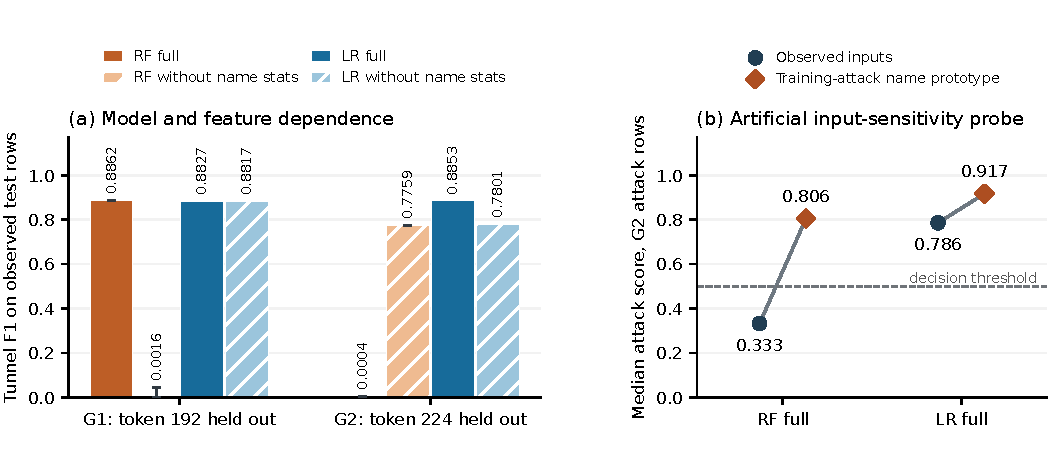
\includegraphics[width=.97\textwidth]{figures/rf_collapse_mechanism.pdf}
\caption{Central CIC mechanism check. (a) Seed-42 test F1 on fixed coarse-token folds; black RF whiskers span the minimum--maximum over five forest seeds. Deleting name statistics reverses RF's fold sensitivity. (b) Median RF/LR attack scores for GROUP-2 attacks before and after artificial substitution of training-attack name medians. The substitution is applied to all test rows; benign effects are in the supplement. Panel (b) measures input sensitivity, not a new detection result.}
\label{fig:mechanism}
\end{figure*}
At seed 42, RF FULL detects five of 26,207 GROUP-2 attacks; LR FULL detects 25,959. Across all five RF seeds, GROUP-2 FULL F1 is \SeedTwoFullMin--\SeedTwoFullMax; without name statistics it is approximately 0.7759, with FPR still 28.11--28.13\%. GROUP-1 FULL stays at \SeedOneFullMin--\SeedOneFullMax, versus \SeedOneNoNameMin--\SeedOneNoNameMax\ without name statistics. FULL-minus-removed F1 is positive on GROUP 1/3 and negative on GROUP 2 at every seed. The supplement retains all 30 results.

It would be incorrect to describe the primary RF as directly learning a rule such as ``\code{sld}=192 implies attack'': \code{sld} is absent from its inputs. Replacing that grouping column while holding indices fixed leaves the entire input matrix unchanged. Instead, the partitions exchange dominant populations with different name statistics. In GROUP 2, training-attack median entropy is 2.675 versus 2.054 at test; the supplied \code{len} median changes from 14 to 11, and \code{subdomain\_length} from 10 to 7. RF's piecewise thresholds respond to these joint distributions differently from LR's scaled linear score.

A concrete path check makes the mechanism inspectable. The most common missed RF input vector occurs 2,192 times among the 26,202 false negatives. Its attack score is 0.345 for RF and 0.796 for LR. Across the forest paths for that vector, entropy, \code{len}, \code{FQDN\_count}, and subdomain length contribute the largest downward terms. In the first tree, a positive PTR branch is followed by \code{FQDN\_count}$\leq24$ and subsequent name-statistic splits, ending at a zero-positive leaf. Full paths and their exact additive check are supplied.

The cohort probe tests whether this explanation extends beyond the example. GROUP-2 attacks have median RF score 0.333 on observed inputs, below the 0.5 decision threshold. Substituting the training-attack name prototype moves that median to 0.806; LR is above threshold both before and after substitution (Fig.~\ref{fig:mechanism}b). The probe also moves benign scores and makes about 29\% of benign rows positive, so it is evidence of name-input reliance, not a remedy. Together, the ablation reversal, feature shift, and tree paths support a model-specific threshold mechanism associated with coarse populations. They do not require a literal token feature.

\subsection{Repetition Is a Distinct Dependency}
The supplied CSV has substantial complete-row repetition and feature-equivalent records carrying opposite labels (Table~\ref{tab:controls}). ROW also permits identical nonlabel vectors across the train/test boundary. Those facts establish dependence opportunities and ambiguity at the supplied feature resolution.

Nevertheless, RF FULL F1 is 0.8864 on ROW and 0.8863 on the exact-vector-disjoint diagnostic. A large duplicate count alone therefore does not explain the high score. The diagnostic partitions different populations and estimates robustness to this particular exclusion; it is not a paired causal estimate of deduplication. The full three-fold results further show that the prominent RF/LR difference persists as a split-sensitive issue: mean FULL F1 is 0.5250 for RF and 0.8043 for LR. Fold heterogeneity, especially RF's GROUP-2 collapse, is more informative than a single mean.

\section{CTU: A Release-Level Representation Mismatch}
\subsection{The Artifact Precedes Our Feature Extraction}
\begin{figure}[t]
\centering
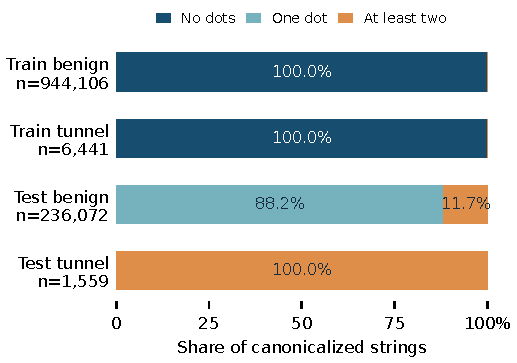
\includegraphics[width=\columnwidth]{figures/ctu_representation_shift.pdf}
\caption{CTU binary subsets after common canonicalization. Every training string is a single label. Only 47 of 236,072 benign test strings have no dots; every tunnel test string has at least two. Original multiclass counts and raw-string checks are in the supplement.}
\label{fig:ctu}
\end{figure}
Checksum-verified original downloads reproduce a systematic mismatch: all training strings lack dots, whereas almost all test strings contain them. This holds across the original normal, DGA, and tunnel classes, before binary filtering. In the canonicalized binary data, the mismatch is visible in Fig.~\ref{fig:ctu}. Counting the original raw normal test strings instead gives 236,027 dotted rows; removing trailing root dots reduces that count by two to 236,025. This normalization detail does not change the result.

The shift changes more than a single dot-count feature. For every binary training row, total length equals both maximum and mean label length. That training identity fails on 237,584 of 237,631 test rows. A model trained on single-label measurements is consequently evaluated on a different combination of lexical measurements. The released split cannot directly support an interpretation of performance under a consistent full-domain representation without auditing or aligning the preprocessing.

\subsection{Deleting Dot Count Does Not Align the Units}
Our LR8 control uses length, dot count, maximum/mean label length, digit/hyphen fractions, entropy, and unique-character fraction. With train-fitted scaling and balanced LR, full-string test F1 is 0.2515. Scoring first labels instead yields 0.1432. First-label extraction is deliberately lossy; it can remove payload-bearing labels and is not a validated repair.

The dot-count input is zero throughout training and has a fitted LR coefficient of exactly zero. Dropping only that input changes \emph{none} of the 237,631 test predictions, under either test representation. This negative control connects the CTU result to the paper's central message: deleting a named feature does not remove a structural distribution difference encoded in the remaining measurements. The problem is a mismatch in what the observations represent.

\subsection{Exposure of Published Pipelines: What Was Checked}
We traced the release to Palau et al.'s 2019 MC-CNN paper \cite{ctupaper}. Its reported per-class test supports match the released test files, making it relevant to investigate that pipeline. At the inspected, pinned commit of the author-associated \emph{deepseq} repository \cite{deepseq}, preprocessing tokenizes characters, then pads/truncates at the end. The classifier defaults to 45 characters; the inspected functions do not remove domain suffixes. As an exposure check, a dot remains within the first 45 raw characters of every dotted normal test string and 1,257 of 1,559 tunnel test strings, while no training string contains one.

This establishes that the release artifact survives that inspected length convention. It does not determine the effect on the original trained MC-CNN: the exact run configuration, vocabulary, model checkpoint, and evaluation trace are not identified by the current code alone. We therefore do not relabel its published score as invalid or reproduce it with our LR controls. The authors' 2020 follow-up describes a new five-tool dataset \cite{palau2020}; its results cannot automatically be assigned the artifact of this three-tool release. The supplement records source hashes, commit, and the boundary between verified exposure and unverified score impact.

\section{Laboratory Support and Shared Interpretation}
LAB normal/tunnel traffic use separate clients, A/AAAA versus NULL, and different zones. GRAPH and the NULL-type control classify all 90 groups correctly; POINT/HYBRID have six false positives. Joint deletion of three suspected graph proxies leaves GRAPH perfect. Median imputation reduces HYBRID false positives to four, linking errors to sparse-group measurements.

All 114 matched SERVFAIL responses and all 96 paired latencies above ten seconds belong to normal traffic; the tunnel has one unmatched query. This contradicts a tunnel-only SERVFAIL hypothesis. These window groups share one tunnel scenario.

Each source supports inference at its observation unit: CIC permits row-level model tests, CTU exposes string-unit inconsistency, and LAB reveals class-aligned acquisition conditions. Korving supports attack-side metadata coverage. These units do not justify cross-source F1 ranking.

\section{Reproducibility, Scope, and AI Use}
The original 50 CIC conditions, additional controls, and 30 seed fits were executed on the project VM with Python 3.12.16 and the locked packages. Independent checks recompute metrics from saved predictions and confirm all six seed-42 RF baselines. Mechanism refits preserve the original labels. RF scores match the earlier Python 3.12.14 execution; small LR score differences leave labels unchanged. Tables use VM outputs. Execution archives, source hashes, numerical comparisons, and environments are retained.

\paragraph{Scope and limitations}
Our CIC findings concern a third-party CSV with unverified packet-to-row lineage. Missing full names, source IPs, and timestamps prevent registrable-domain/time/session holdouts or a protocol-matched reconstruction of the published hybrid. Coarse-token folds and forest seeds measure sensitivity; exact-vector exclusion controls one dependency, and synthetic substitution probes model inputs. LAB and Korving each cover one attack scenario. CTU's release-level mismatch does not quantify causal damage to an unavailable neural checkpoint.

\paragraph{Code and data availability}
Source, frozen splits, and reproduction instructions are available at \url{https://github.com/QuangApollo/iam302t-dns-shortcut-audit}. The LMS submission includes complete row-level predictions and original VM evidence. Checksum-pinned scripts retrieve the public datasets.


\paragraph{AI-use disclosure}
ChatGPT (OpenAI) assisted with wording, code drafting, literature lookup, diagnostic design, and figures. Numerical claims derive from executed scripts and saved outputs, with validation in the package. Authors are responsible for reviewing the material, scientific interpretation, and final submission.

\section{Conclusion}
Column deletion is not equivalent to information removal. TTL retains type information, and name-statistic thresholds produce different RF/LR behavior on coarse-token splits. RF's ablation reversal persists across five forest seeds; verified paths locate its failure in numeric inputs. The exact-vector control distinguishes repetition from this mechanism. CTU shows why dropping dot count cannot align train tokens with test domains. A defensible ablation claim needs an explicit feature inventory, a residual-information test, and a split matching the intended inference.

\begin{thebibliography}{19}
\bibitem{nadler} A. Nadler, A. Aminov, and A. Shabtai, ``Detection of malicious and low throughput data exfiltration over the DNS protocol,'' \emph{Computers \& Security}, vol. 80, pp. 36--53, 2019, doi:10.1016/j.cose.2018.09.006.
\bibitem{geirhos} R. Geirhos et al., ``Shortcut learning in deep neural networks,'' \emph{Nature Machine Intelligence}, vol. 2, pp. 665--673, 2020, doi:10.1038/s42256-020-00257-z.
\bibitem{arp} D. Arp et al., ``Dos and Don'ts of Machine Learning in Computer Security,'' in \emph{31st USENIX Security Symposium}, pp. 3971--3988, 2022.
\bibitem{zhao} Y. Zhao, L. Li, H. Wang, H. Cai, T. F. Bissyandé, J. Klein, and J. Grundy, ``On the impact of sample duplication in machine-learning-based Android malware detection,'' \emph{ACM Trans. Softw. Eng. Methodol.}, vol. 30, no. 3, art. 40, 2021, doi:10.1145/3446905.
\bibitem{tesseract} F. Pendlebury, F. Pierazzi, R. Jordaney, J. Kinder, and L. Cavallaro, ``TESSERACT: Eliminating experimental bias in malware classification across space and time,'' in \emph{28th USENIX Security Symposium}, pp. 729--746, 2019.
\bibitem{engelen} G. Engelen, V. Rimmer, and W. Joosen, ``Troubleshooting an intrusion detection dataset: the CICIDS2017 case study,'' in \emph{IEEE Security and Privacy Workshops}, pp. 7--12, 2021, doi:10.1109/SPW53761.2021.00009.
\bibitem{cicpaper} S. Mahdavifar et al., ``Lightweight hybrid detection of data exfiltration using DNS based on machine learning,'' in \emph{11th Int. Conf. Communication and Network Security}, pp. 80--86, 2021, doi:10.1145/3507509.3507520.
\bibitem{ctupaper} F. Palau, C. Catania, J. Guerra, S. Garcia, and M. Rigaki, ``Detecting DNS threats: A deep learning model to rule them all,'' in \emph{XX Simposio Argentino de Inteligencia Artificial, JAIIO 48}, pp. 90--101, 2019. [Online]. Available: \url{https://sedici.unlp.edu.ar/handle/10915/87859}.
\bibitem{ctudata} F. Palau et al., ``DNS Threats Dataset, Version 1,'' Zenodo, 2022, doi:10.5281/zenodo.6508640.
\bibitem{cicdata} Canadian Institute for Cybersecurity, ``CIC-Bell-DNS-EXF-2021 dataset,'' University of New Brunswick. [Online]. Available: \url{https://www.unb.ca/cic/datasets/dns-exf-2021.html}. Accessed: Nov. 4, 2026.
\bibitem{cicmirror} S. Rajan, ``Feature-Based DNS Traffic Dataset for Heavy Attack Detection,'' Zenodo, v1, Jan. 2026, doi:10.5281/zenodo.18139853.
\bibitem{psl} Mozilla Foundation, ``Public Suffix List.'' [Online]. Available: \url{https://publicsuffix.org/}. Accessed: Nov. 4, 2026.
\bibitem{korving} F. Korving, ``DNS Tunneling Dataset,'' GitHub. [Online]. Available: \url{https://github.com/Korving-F/dns-tunnel-dataset}. Accessed: Nov. 4, 2026.
\bibitem{sklearnpitfalls} Scikit-learn developers, ``Common pitfalls and recommended practices.'' [Online]. Available: \url{https://scikit-learn.org/stable/common_pitfalls.html}. Accessed: Nov. 4, 2026.
\bibitem{deepseq} C. Catania et al., ``Deepseq: Deep learning sequence classifier,'' GitHub, inspected commit \code{769e3466f901}, accessed Nov. 4, 2026. [Online]. Available: \url{https://github.com/harpomaxx/deepseq}.
\bibitem{palau2020} F. Palau, C. Catania, J. Guerra, S. Garcia, and M. Rigaki, ``DNS tunneling: A deep learning based lexicographical detection approach,'' arXiv:2006.06122v2, 2020, doi:10.48550/arXiv.2006.06122.
\end{thebibliography}

\end{document}
